\subsection{拓扑与初始资金配置的四臂补充分析}

在已有父图上开展事后分析，固定需求感知构造DA和FHS5拓扑，分别使用节点预算均匀初态U和原优化初态O，形成DA-U、FHS5-U、DA-O和FHS5-O四臂。每节点预算均为120，O臂复用原受核验结果，U臂使用同一留出请求及请求级路由票据。配置变化可改变超边资金总额，因此这里并非固定每条超边资金的纯拓扑因果干预。

对两个服务终点分别计算
\begin{equation}
\begin{aligned}
\Delta_U&=\overline Z_{\mathrm{DA-U}}-\overline Z_{\mathrm{FHS5-U}},\\
\Delta_O&=\overline Z_{\mathrm{DA-O}}-\overline Z_{\mathrm{FHS5-O}},\\
\Gamma&=\Delta_O-\Delta_U,
\end{aligned}\label{eq:s5-interaction}
\end{equation}
其中$Z$取归一化受限无路径时间或窗口内失败指示。$\Gamma$是两拓扑各自O减U之差，由共享重抽样直接计算，不以一项区间含零、另一项不含零判断交互。

每相位、每规模60父图，3模型各20；7条轨迹先在父图内平均，模型均值等权。四臂与两终点共用模型分层整父图重抽样索引，20\,000次重抽样形成点态95\% percentile区间。全部80项合并比较均报告，未作多重比较校正。相位标签沿用原数据，这不是新的预注册或盲确认实验；完整统计方法及子范围描述见补充材料。

均匀初态下，30节点DA减FHS5的时间差在正式、确认相位分别为0.002077和0.001171；240节点两相位均为0。完整拓扑差与交互见补充图S2，零宽经验区间不证明总体等效。图\ref{fig:s5-initialization}展示各拓扑的O减U：16个相位、规模及拓扑条件中，时间差点估计15负、1正，不是16个独立重复或统计检验。确认相位240节点两拓扑的时间差均为$-0.005575$，点态区间$[-0.012888,-0.000705]$；失败风险均增加1.667个百分点，点态区间$[0.238,3.571]$个百分点。

\begin{figure*}[t]\centering
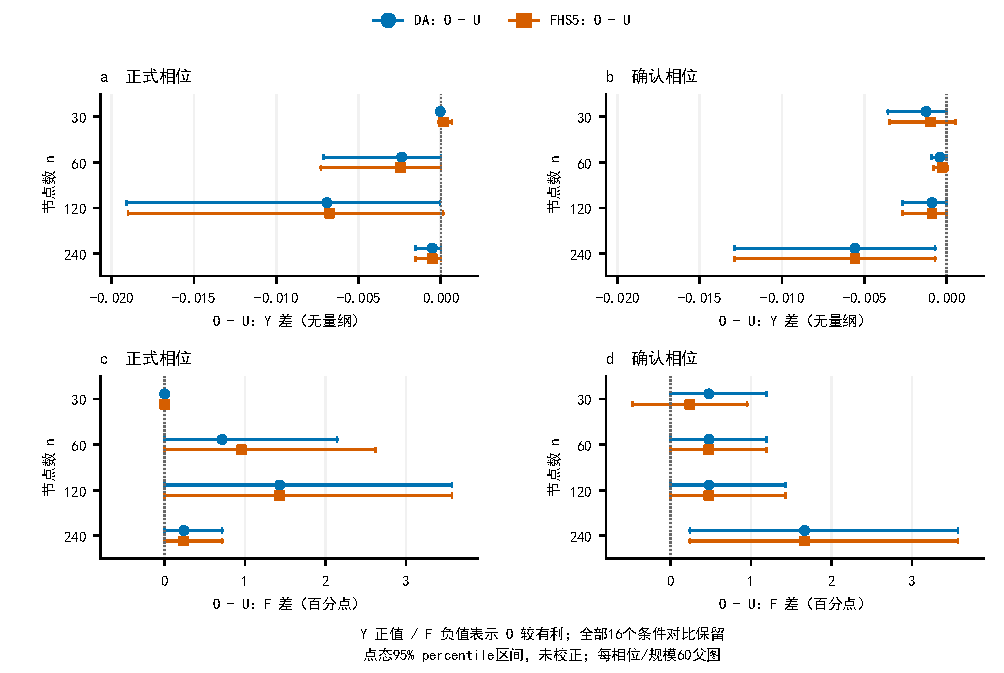
\includegraphics[width=170mm]{figures/s5-initialization.pdf}
\caption{固定拓扑内的初态对比。a、b为正式、确认相位的归一化时间差；c、d为失败风险差（百分点）。圆点与方块分别为DA和FHS5的O减U估计，横线为点态、未校正95\%区间；每相位、每规模60父图，3模型各20，7条轨迹先在父图内汇总。时间差正值、风险差负值表示O较有利；全部条件保留，源数据见补充材料。}\label{fig:s5-initialization}
\end{figure*}

原优化初态在已观察条件中并非普遍有利。结构搜索的静态需求目标与资金配置的有限训练情景字典序评分，都不保证留出终点改善；当前数据也未识别差距的机制。超图相对二元参照的主结果、DA相对FHS5的搜索增量及O相对U的配置增量属于不同估计对象，不能相互替代。
